\cxset{style42/.style={
 name=chapter,
 chapter opening=right,
 numbering= arabic,
 number font-size=huge,
 number before=,
 number after=\hrule,
 number display=block,
 number float=left,
 number position=rightname,
 chapter display=block,
chapter float=left,
 chapter before=\vspace*{10pt},
 number after=,
 chapter after=,
 number color= gray,
 title font-family=sffamily,
 title font-color= black!80,
 title font-weight=,
 title font-size=Huge,
 title before=,
 title after=,
 title margin top=10pt,
 title margin bottom=10pt,
 chapter title text-align=left,
 chapter title align=left,
 author block=false,
 section numbering=none,
 epigraph width=0.85\textwidth,
 epigraph text align=left,
 epigraph source align=right,
 epigraph rule width=0pt,
 epigraph afterskip=30pt,
}}

\cxset{style42}
\chapter{Introduction to Style Forty Two}

\epigraph{Tell me, O Muse, of that ingenious hero who trawled far and wide after he had
sacked the famous town of Troy. Many cities did he visit, and many were the nations with whose manners
and customs he was acquainted; moreover he suffered much by sea while trying to save his own life and bring
his men safely home \ldots }{Homer, \textit{The Odyssey}}

Style 42 is shown in the following figure:

\begin{figure}[ht]
\centering
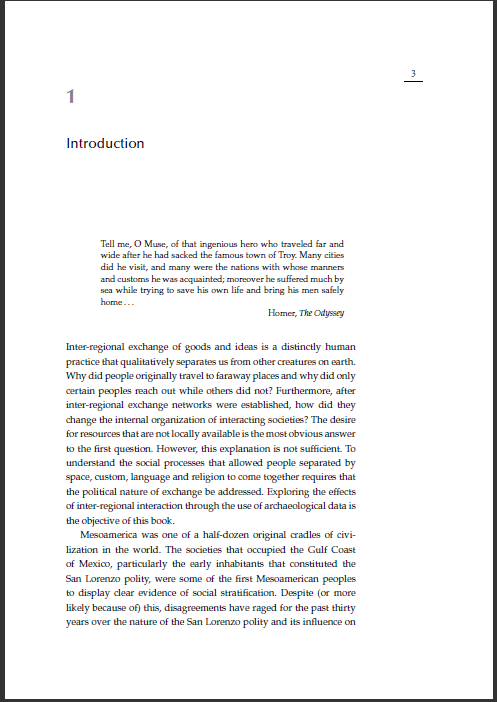
\includegraphics[width=0.6\textwidth]{./chapters/chapter42.png}
\end{figure}

The distinguishing characteristics of this chapter are that it has an epigraph and is composed of very simple stylistic elements. The epigraph is placed quite a bit lower than the chapter title. The heading style is just the page number and underlined.



